\documentclass[3p,times,procedia]{elsarticle}
\flushbottom

\usepackage{ecrc}
\usepackage[bookmarks=false]{hyperref}
\hypersetup{hidelinks}

\usepackage{amsmath}
\usepackage{amssymb,amsfonts}
\usepackage{algorithmic}
\usepackage{algorithm}
\usepackage{graphicx}
\usepackage{textcomp}
\usepackage{xcolor}
\usepackage{booktabs}
\usepackage{multirow}
\usepackage{url}
\usepackage{acronym}
\usepackage[section]{placeins}

\volume{00}
\firstpage{1}
\journalname{Procedia Computer Science}
\runauth{A. Gargouri et al.}
\jid{procs}

\acrodef{hrc}[HRC]{Human-Robot Collaboration}
\acrodef{icl}[ICL]{Incremental and Continual Learning}
\acrodef{flair}[FLAIR]{FiLM-based Learning with Adaptive Importance and Replay}
\acrodef{film}[FiLM]{Feature-wise Linear Modulation}
\acrodef{ewc}[EWC]{Elastic Weight Consolidation}
\acrodef{derpp}[DER++]{Dark Experience Replay++}
\acrodef{l2p}[L2P]{Learning to Prompt}
\acrodef{si}[SI]{Synaptic Intelligence}
\acrodef{er}[ER]{Experience Replay}
\acrodef{agem}[A-GEM]{Average Gradient Episodic Memory}
\acrodef{mlp}[MLP]{Multilayer Perceptron}
\acrodef{mse}[MSE]{Mean Squared Error}
\acrodef{acc}[ACC]{Average Accuracy}
\acrodef{bwt}[BWT]{Backward Transfer}
\acrodef{fwt}[FWT]{Forward Transfer}
\acrodef{harmonic}[HARMONIC]{Human And Robot Multimodal Observations of Natural Interactive Collaboration}

\begin{document}
\begin{frontmatter}

\dochead{30th International Conference on Knowledge-Based and Intelligent Information \& Engineering Systems (KES 2026)}

\title{A Combined Incremental Learning Algorithm for Human-Robot Collaboration}

% \author{
% \IEEEauthorblockN{1\textsuperscript{st} Ameur Gargouri}
% \IEEEauthorblockA{\textit{ESME Research Lab} \\
% \textit{ATISP Laboratory, ENET'Com, University of Sfax}\\
% Ivry-sur-Seine, France / Sfax, Tunisia \\
% gargouri.ameur@enis.tn}
% \and
% \IEEEauthorblockN{2\textsuperscript{nd} Mohamed Karray}
% \IEEEauthorblockA{\textit{ESME Research Lab} \\
% Ivry-sur-Seine, France \\
% ORCID: 0000-0001-7293-8696}
% \and
% \IEEEauthorblockN{3\textsuperscript{rd} Mohamed Ksantini}
% \IEEEauthorblockA{\textit{ATISP Laboratory, ENET'Com, University of Sfax}\\
% Sfax, Tunisia \\
% mohamed.ksantini@ipeis.usf.tn \\
% ORCID: 0000-0002-9928-8643}
% }

\author[a,b]{Ameur Gargouri}
\author[b]{Mohamed Karray*}
\author[a]{Mohamed Ksantini}

\address[a]{ATISP Lab, ENET'Com, University of Sfax, Sfax, Tunisia}
\address[b]{ESME Research Lab, Ivry-sur-Seine, France}

\begin{abstract}
\ac{hrc} in person-assistance scenarios requires learning natural collaborative behaviors from human demonstrations, rather than repeating fixed routines as in many industrial settings. These behaviors are more complex and non-stationary, needing \ac{icl} methods. In fact, each new user introduces distinct interaction patterns, and the robot's system must continuously interpret multimodal inputs whose cross-modal relationships can drift across users. Existing such learning methods typically rely on either regularization or replay alone, which limits their ability to balance adaptation to new users and retention of prior skills. We propose, in this paper, a hybrid incremental learning algorithm, FLAIR, that combines task-conditioned modulation, task-aware experience replay with dark-knowledge distillation, online Fisher-based importance regularization with retroactive boosting, and multi-head output blending. We train and evaluate FLAIR on a multimodal \ac{hrc} dataset (joystick commands, robot joint states, and end-effector signals) collected from human operators in shared-autonomy assistance tasks. Results show that FLAIR achieves the best \ac{acc} (\ac{acc} = 0.690), surpassing existing incremental learning algorithms.
\end{abstract}

\begin{keyword}
human-robot collaboration \sep incremental learning \sep multimodal learning \sep assistive robotics
\end{keyword}
%\cortext[cor1]{Corresponding author. Tel.: +0-000-000-0000 ; fax: +0-000-000-0000.}
\end{frontmatter}

%\correspondingauthor[*]{Corresponding author. Tel.: +0-000-000-0000 ; fax: +0-000-000-0000.}
%\email{author@institute.xxx}
\newpage

%===================================================================
\section{Introduction}
%===================================================================

\acp{hrc} are increasingly deployed in assistive robotics, teleoperation, and rehabilitation, where robots must adapt to diverse users while maintaining reliable behavior over time~\cite{javdani2018shared, reddy2018shared, selvaggio2021autonomy}. Unlike many structured industrial workflows where tasks are well-defined and stationary, person-assistance interactions are natural and user-dependent, with larger variability in intent and motion patterns. In such long-running deployments, new operators are encountered sequentially, and each operator exhibits distinct motor preferences. This requires incremental learning algorithms that must \emph{adapt} to new users without \emph{forgetting} previously learned collaboration behaviors.

This type of learning scenarios involves input multimodality, which in \ac{hrc} denotes the joint modeling of heterogeneous signals that capture complementary aspects of interaction, such as human intent inputs (e.g., joystick commands), robot proprioceptive state (e.g., joint positions), and task-space motion cues (e.g., end-effector pose/trajectory).% The robot's system must preserve useful cross-modal representations as user-specific interaction dynamics evolve over time.

This setting is a clear case of \emph{catastrophic forgetting}~\cite{delange2022continual}, where neural networks lose performance on previously learned tasks as training continues on new tasks. In \ac{icl}, there are three main types of mitigation strategies: regularization-based approaches, such as \ac{ewc}~\cite{kirkpatrick2017overcoming}, that penalize updates to parameters important for prior tasks; replay-based approaches, such as \ac{derpp}~\cite{buzzega2020dark}, that mix current-task data with buffered past samples; and architecture-based approaches, such as \ac{l2p}~\cite{wang2022l2p}, that allocate task-specific representational capacity to reduce interference.

Each family addresses only a subset of the stability-plasticity trade-off. Regularization-based approaches improve retention but may reduce plasticity for incoming tasks. Replay-based approaches improve memory of prior data but depend strongly on buffer composition and sampling policy, without explicitly constraining parameter drift. Architecture-based approaches reduce interference by task separation, yet their parameter growth can limit scalability as the number of users/tasks increases.

For assistive HRC, this limitation is amplified by multimodal learning demands: the algorithm must preserve cross-modal coordination (human intent signals and robot state dynamics) while adapting to new users. This motivates the need for a stronger incremental learning algorithm tailored to realistic person-assistance settings.

To enable robust adaptation to human intent and gesture variability, we propose \ac{flair}, an integrated hybrid incremental learning algorithm for sequential policy adaptation in \ac{hrc}. This algorithm is trained on the \ac{harmonic} dataset~\cite{newman2022harmonic}, collected from 24 users, imitating assistive eating. The main contributions are:

\begin{enumerate}
    \item A hybrid algorithm that jointly integrates per-task \ac{film} conditioning~\cite{perez2018film}, task-aware experience replay with dark knowledge distillation, online Fisher-based importance regularization, retroactive importance boosting (RetroBoost), FiLM warm-start initialization, and forgetting-proportional adaptive replay weighting.
    \item Multi-head output blending embedded in the same unified training objective to balance per-task specialization with cross-task knowledge sharing.
    %\item An empirical evaluation on a 10-user sequential multimodal HRC benchmark of natural assistive tasks showing that FLAIR surpasses even the Joint Training upper bound (ACC = 0.690 vs.\ 0.644) with near-zero forgetting (F = 0.017) and minimal memory overhead (1.28 MB).
\end{enumerate}

%===================================================================
\section{Related Works}
%===================================================================

%\subsection{Human-Robot Collaboration and Shared Autonomy}

Research in assistive robotics can be grouped into three main areas: human-robot collaboration, shared autonomy, and multimodal learning. Together, these directions show that assistive systems must balance safe, intent-aware interaction with robust fusion of heterogeneous signals, while adapting to diverse users over time. 
%The following studies illustrate how these three directions have evolved and where important limitations remain for long-horizon incremental adaptation.

%Javdani et al.~\cite{javdani2018shared} introduced hindsight-optimization-based shared autonomy for robotics systems, where autonomous assistance is selected by optimizing expected user outcomes under uncertainty about intent. Their formulation establishes a principled decision-theoretic basis for assistance, but it does not explicitly address long-horizon sequential user adaptation with forgetting constraints.

%Reddy et al.~\cite{reddy2018shared} presented a deep reinforcement learning formulation of shared autonomy that learns arbitration policies directly from interaction feedback. This line of work improves adaptive control quality, yet it mainly optimizes task performance per training regime rather than preserving previously acquired user-specific behaviors across many users.

Selvaggio et al.~\cite{selvaggio2021autonomy} surveyed autonomy levels in physical human-robot interaction and highlighted design trade-offs between safety, transparency, and adaptation. Importantly, the survey emphasizes that adaptation mechanisms in assistive interaction must remain reliable and interpretable, which becomes harder when the user population grows over time.

Losey et al.~\cite{losey2018assistive} presented a review of shared control in physical human-robot interaction, with a structured analysis of three core components: intent detection, arbitration between human and robot commands, and communication/feedback to the user. Their work clarifies design trade-offs and evaluation criteria for assistive shared autonomy, and provides a conceptual foundation for building reliable human-in-the-loop controllers. %However, the paper does not address long-horizon sequential adaptation across many users, where retaining previously learned user-specific behaviors becomes a central requirement.

More recently, Thumm et al.~\cite{thumm2024hrgym} proposed Human-Robot Gym as a benchmarking environment for reinforcement learning in collaborative settings, enabling standardized comparison across HRC control strategies. Such benchmarks strengthen reproducibility, but they also reveal that most current evaluations still focus on per-task adaptation quality rather than long-term incremental retention.

%Collectively, these works show that person-assistance HRC increasingly depends on intent-aware control, multimodal representation learning, and robust adaptation under user variability. However, an important gap remains: existing approaches are rarely designed as integrated incremental-learning systems that jointly optimize adaptation to new users and retention of prior user-specific motor collaboration patterns.

%Recent comprehensive surveys and empirical analyses further contextualize our approach. 
Serra-Perello and Ortiz~\cite{serra2025incremental} provide an extensive taxonomy and experimental evaluation of incremental learning methodologies, highlighting practical trade-offs between replay, regularization, and architecture-based strategies. 

A recent review by Bako, J. and Kalita, J~\cite{springer2026review} synthesizes recent advances in continual learning and discusses deployment considerations that are particularly relevant for robotics and multimodal systems.

Building on this state of the art, we propose FLAIR, a unified incremental learning algorithm that addresses catastrophic forgetting in sequential multimodal HRC while keeping memory usage practical and performance strong across seen users. Taken together, these references motivate integrated hybrid methods that combine regularization, replay, and task-conditioned architectural adaptation in a single learning system.
%Our contribution directly addresses this gap by proposing FLAIR as a unified hybrid incremental algorithm that combines task-conditioned modulation, task-aware replay, and importance-weighted regularization in a single training framework. This design targets the central HRC failure mode highlighted above, namely catastrophic forgetting under sequential multimodal user adaptation, while preserving practical memory usage and maintaining strong predictive performance across all seen users.

% \subsection{Incremental and Continual Learning}

% Continual and incremental learning methods aim to learn task sequences $\{T_1, T_2, \ldots, T_N\}$ without catastrophic forgetting.

% The authors in~\cite{kirkpatrick2017overcoming} proposed \ac{ewc}, which constrains parameter updates by Fisher-weighted penalties to preserve knowledge from previous tasks.

% In~\cite{schwarz2018progress}, the work extended \ac{ewc} to online settings by accumulating importance estimates over time, improving scalability in long task streams.

% The approach in~\cite{zenke2017continual} introduced \ac{si}, which estimates parameter importance from contribution to loss reduction during training trajectories.

% The work presented in~\cite{chaudhry2019tiny} studied \ac{er} with limited memory and showed that carefully managed episodic buffers can remain competitive.

% In~\cite{buzzega2020dark}, the authors introduced \ac{derpp}, combining replay with logit distillation to stabilize representations across tasks.

% A different perspective appears in~\cite{chaudhry2018efficient}, where \ac{agem} enforces gradient constraints using memory samples rather than replaying all past data directly.

% The authors in~\cite{wang2022l2p} proposed \ac{l2p}, an architecture-oriented strategy that uses task-specific prompts to adapt models with reduced interference.

% In~\cite{douillard2022dytox}, the authors developed DyTox with dynamic token expansion in transformers to incrementally allocate representational capacity.

% The study in~\cite{prabhu2020gdumb} questioned progress in continual learning by showing that strong replay-only baselines can be surprisingly competitive under fair protocols.

% The work in~\cite{caccia2022new} analyzed abrupt representation changes and introduced mitigation strategies that improve online continual learning stability.

% For robotics specifically,~\cite{auddy2023clfd} demonstrated continual learning from demonstrations to accumulate robot skills across sequentially presented tasks.

% In~\cite{guerdan2023federated}, the authors explored federated continual learning for socially aware robotics, targeting distributed interaction data without centralizing all user trajectories.

% The authors in~\cite{fan2024continualhrc} discussed continual learning pipelines tailored to human-robot collaboration, emphasizing adaptive support in evolving collaborative workflows.

% Taken together, these references motivate integrated hybrid methods that combine regularization, replay, and task-conditioned architectural adaptation in a single learning system.

% \subsection{FiLM Conditioning}

% In~\cite{perez2018film}, the authors introduced \ac{film}, an affine feature modulation mechanism $\text{FiLM}(h)=\gamma\cdot h+\beta$ conditioned on contextual signals. This conditioning strategy is particularly relevant to our setting because it enables task-specific adaptation while retaining a shared backbone.
%===================================================================
\section{Methodology}
%===================================================================
\subsection{Problem Formulation}

We consider the task-incremental learning setting. A sequence of $N$ tasks $\{T_1, \ldots, T_N\}$ arrives one at a time, where each task $T_i$ corresponds to a distinct human operator in a natural assistive interaction. For task $T_i$, the agent observes multimodal inputs (joystick commands, joint positions, and end-effector positions; observation $o \in \mathbb{R}^{d_o}$) and must predict the corresponding joint velocity commands (action $a \in \mathbb{R}^{d_a}$). The goal is to learn a policy $\pi_\theta$ that performs well on \emph{all} tasks after sequentially training on each, while maintaining robust cross-modal representations as user dynamics evolve.

\subsection{Proposed Architecture: FLAIR}

\ac{flair} uses a shared \ac{mlp} backbone with per-task FiLM conditioning layers. The architecture consists of:
This displayed equation shows how FiLM implements task-specific modulation: a shared linear transform is passed through a nonlinearity and then scaled and shifted by task-dependent parameters. The simple affine modulation enables strong task specialization without duplicating the full backbone, keeping memory and compute efficient.
\begin{equation}
    h^{(l)} = \text{Dropout}\left(\gamma_t^{(l)} \cdot \text{ReLU}\left(W^{(l)} h^{(l-1)} + b^{(l)}\right) + \beta_t^{(l)}\right)
    \label{eq:film_layer}
\end{equation}
where $W^{(l)}, b^{(l)}$ are \emph{shared} backbone weights and $\gamma_t^{(l)}, \beta_t^{(l)}$ are \emph{task-specific} FiLM parameters. 

The next equation shows how final predictions combine shared knowledge with a task-specialized head: a weighted blend lets the model fall back on general features while using task-specific corrections when needed.
\begin{equation}
    \hat{a} = (1 - \alpha_h) \cdot f_{\text{shared}}(h^{(L)}) + \alpha_h \cdot f_t(h^{(L)})
    \label{eq:multi_head}
\end{equation}
where $\alpha_h = 0.3$ is the head blending coefficient.

After training on task $t$, its FiLM parameters and task head are \emph{frozen}, preventing retroactive modification and ensuring stability.

Fig.~\ref{fig:architecture} illustrates FLAIR's design: data flows through FiLM-conditioned shared layers that are modulated by task-specific parameters ($\gamma_t, \beta_t$), then through two output heads (shared and per-task) that are adaptively blended. Three auxiliary mechanisms support incremental learning: a task-aware replay buffer with adaptive weighting, Fisher-based importance regularization with retroactive boosting, and FiLM warm-start initialization. Frozen components after training are marked with \textit{snowflake} icons.
\begin{figure}[!t]
    \centering
    
\includegraphics[width=\columnwidth]{flair_architecture.pdf}
    \caption{FLAIR architecture and auxiliary mechanisms}
    \label{fig:architecture}
\end{figure}
\FloatBarrier
\subsubsection{Training Objective}

The total training loss for task $t$ combines four terms: one that fits the current task, two that preserve previous behavior via replay and logit consistency, and a regularizer that prevents destructive parameter updates. Together these terms balance plasticity (learning new tasks) and stability (preserving previous tasks), which is the core objective in continual learning.
\begin{equation}
    \mathcal{L} = \mathcal{L}_{\text{task}} + \alpha \mathcal{L}_{\text{logit}} + \beta \mathcal{L}_{\text{replay}} + \frac{\lambda}{2} \mathcal{L}_{\text{reg}}
    \label{eq:total_loss}
\end{equation}
where:

\textbf{Task loss:} Standard \ac{mse} on the current task's data. This term drives the model to fit the current task's supervisory signal and is the primary driver of plasticity during task-specific training.
\begin{equation}
    \mathcal{L}_{\text{task}} = \frac{1}{|B_t|}\sum_{(o,a) \in B_t} \|\pi_\theta(o; t) - a\|^2
\end{equation}
\textbf{Logit distillation loss:} For replayed samples $(o_r, t_r)$ from the buffer, consistency is encouraged with stored logits $\hat{a}_r$. This term preserves the model's previous outputs for past inputs even if internal representations change, which helps maintain behavior when representations drift.
\begin{equation}
    \mathcal{L}_{\text{logit}} = \frac{1}{|B_r|}\sum_{(o_r, t_r) \in B_r} w_r \|\pi_\theta(o_r; t_r) - \hat{a}_r\|^2
\end{equation}
where $w_r$ is the adaptive replay weight (Section~\ref{sec:adaptive}).

\textbf{Replay target loss:} Direct MSE on replayed ground-truth actions. This term explicitly rehearses previous behavior by training the model to reproduce ground-truth actions for past samples, counteracting forgetting.
\begin{equation}
    \mathcal{L}_{\text{replay}} = \frac{1}{|B_r|}\sum_{(o_r, a_r, t_r) \in B_r} w_r \|\pi_\theta(o_r; t_r) - a_r\|^2
\end{equation}
\textbf{Importance regularization:} Fisher-based penalty on shared parameters. This penalty discourages changes to parameters deemed important for previously learned tasks; the Fisher-derived importance $\Omega_i$ weights how strongly each parameter is anchored to its prior value, thereby protecting critical components of the shared backbone.
\begin{equation}
    \mathcal{L}_{\text{reg}} = \sum_{i} \Omega_i (\theta_i - \theta_i^*)^2
    \label{eq:importance_reg}
\end{equation}
where $\Omega_i$ is the cumulative importance and $\theta_i^*$ is the anchor value after the previous task.

\subsubsection{Task-Aware Replay Buffer}

Unlike standard replay buffers, FLAIR stores the \emph{task identity} alongside each sample: $(o, a, \hat{a}, t)$. During replay, each sample is routed through its original task's FiLM parameters, ensuring the correct feature modulation is applied. This is critical because shared backbone features are modulated differently for each task; replaying a sample without the correct FiLM routing would produce incorrect gradients.

\subsubsection{Retroactive Importance Boosting (RetroBoost)}

Standard online EWC accumulates importance as $\Omega^{(t)} = \gamma \Omega^{(t-1)} + F^{(t)}$, where $F^{(t)}$ is the Fisher information for task $t$, augmented with a retroactive boost to gradually increase protection as the task set grows. Intuitively, the shared backbone accrues more responsibilities over time, so anchoring should strengthen accordingly.
\begin{equation}
    \Omega^{(t)} \leftarrow \left(1 + 0.1 \cdot |\text{completed tasks}|\right) \cdot \Omega^{(t)}
\end{equation}
This multiplier increases regularization proportionally to the number of learned tasks, reducing the chance that new updates erase earlier capabilities.

\subsubsection{FiLM Warm-Start}

When a new task $t$ arrives, the cosine similarity is computed between its input statistics (mean and standard deviation of observations) and those of all previously learned tasks. The most similar prior task is selected to initialize FiLM parameters, which typically reduces convergence time and early catastrophic interference by starting from a reasonable, task-appropriate modulation.
\begin{equation}
    t^* = \arg\max_{t' \in \text{completed}} \cos\left([\mu_t; \sigma_t], [\mu_{t'}; \sigma_{t'}]\right)
\end{equation}
\begin{equation}
    \gamma_t^{(l)} \leftarrow \gamma_{t^*}^{(l)}, \quad \beta_t^{(l)} \leftarrow \beta_{t^*}^{(l)}
\end{equation}

This warm-start strategy is particularly effective when users exhibit similar interaction statistics, as it leverages prior task structure rather than learning from scratch.

\subsubsection{Adaptive Replay Weighting}
\label{sec:adaptive}

Standard replay samples uniformly from the buffer. FLAIR instead biases replay towards tasks that show the largest drop from their best achieved performance, focusing rehearsal where it will most reduce forgetting. Concretely, the replay weight increases linearly with the gap between peak and current R\textsuperscript{2}, prioritizing samples from weakened tasks.
\begin{equation}
    w_r = 1 + 5 \cdot \max\left(0, R^2_{\text{peak}}(t_r) - R^2_{\text{current}}(t_r)\right)
\end{equation}
Tasks experiencing greater forgetting (larger gap between peak and current performance) receive proportionally more replay emphasis.

\subsubsection{Algorithmic Visualization}

Algorithm~\ref{alg:flair} summarizes the full FLAIR incremental training pipeline, including FiLM warm-start, task-aware replay, adaptive replay weighting, and Fisher-based regularization with RetroBoost.

\begin{algorithm}[h!]
\caption{FLAIR Incremental Training Procedure}
\label{alg:flair}
\begin{algorithmic}[1]
\STATE \textbf{Input:} task sequence $\{T_1, \ldots, T_N\}$, shared parameters $\theta$, replay buffer $\mathcal{M}$
\STATE \textbf{Initialize:} task statistics store, importance weights $\Omega \leftarrow 0$, anchor parameters $\theta^* \leftarrow \theta$
\FOR{$t = 1$ to $N$}
    \IF{$t > 1$}
        \STATE Compute task similarity statistics and warm-start $(\gamma_t, \beta_t)$ from most similar prior task
    \ELSE
        \STATE Initialize $(\gamma_t, \beta_t)$ to identity
    \ENDIF
    \FOR{each training mini-batch $B_t$ from task $T_t$}
        \STATE Sample replay mini-batch $B_r$ from $\mathcal{M}$ with stored task IDs
        \STATE Route each replay sample through its original task FiLM branch
        \STATE Compute adaptive replay weights $w_r \leftarrow 1 + 5\max(0, R^2_{\mathrm{peak}} - R^2_{\mathrm{current}})$
        \STATE Compute total loss:
        \STATE \hspace{1.0em}$\mathcal{L} \leftarrow \mathcal{L}_{\mathrm{task}} + \alpha\mathcal{L}_{\mathrm{logit}} + \beta\mathcal{L}_{\mathrm{replay}} + \frac{\lambda}{2}\mathcal{L}_{\mathrm{reg}}$
        \STATE Update $\theta$, $(\gamma_t, \beta_t)$, and task head parameters via backpropagation
        \STATE Store sampled current-task examples and logits $(o, a, \hat{a}, t)$ in $\mathcal{M}$
    \ENDFOR
    \STATE Estimate Fisher information $F^{(t)}$ on task $T_t$
    \STATE Update cumulative importance: $\Omega \leftarrow \gamma\Omega + F^{(t)}$
    \STATE Apply RetroBoost: $\Omega \leftarrow (1 + 0.1\cdot |\mathrm{completed\ tasks}|)\Omega$
    \STATE Set anchor parameters: $\theta^* \leftarrow \theta$
    \STATE Freeze task-specific FiLM parameters and task head for task $t$
\ENDFOR
\STATE \textbf{Output:} trained FLAIR model with shared backbone, frozen task-specific FiLM modules, and replay memory
\end{algorithmic}
\end{algorithm}


%===================================================================
\subsection{Used dataset}
%===================================================================

%\subsection{Dataset}

We use the \acs{harmonic} dataset~\cite{newman2022harmonic}, a multimodal human-robot interaction dataset collected from participants controlling a Kinova MICO robotic arm positioned on a table, with a food tray placed in front of the arm (Fig~\ref{fig:experiment}). Each participant holds a 3D joystick controller to teleoperate the robot during natural feeding tasks. The shared-autonomy system records data synchronously at the robot's control frequency: joystick inputs from the human operator, proprioceptive joint angles and velocities from the robot, and end-effector pose. This multimodal measurement captures both the human intent (via joystick) and the robot state, reflecting the natural diversity of control strategies and individual behavioral differences across users. Such heterogeneous interaction patterns form the basis for studying incremental learning and user-specific adaptation.

\begin{figure}[!t]
    \centering
    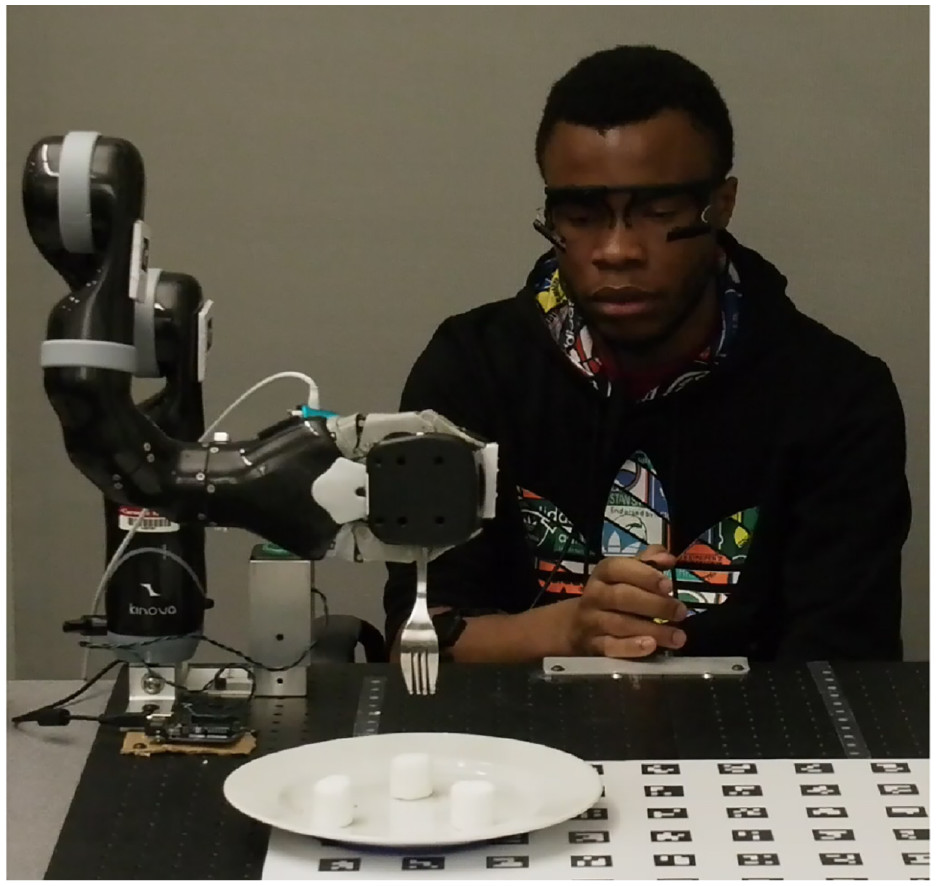
\includegraphics[scale=0.7]{fig1.jpg}
        \caption{Experimental setup: shared autonomy assistive eating task~\cite{newman2022harmonic}}
    \label{fig:experiment}
\end{figure}
\FloatBarrier

\subsubsection{Feature Extraction}

From each trial, we extract three input modalities recorded at the robot's control frequency:

\textbf{Joystick commands} (3D): user input axes $(x, y, z)$; \textbf{Joint positions} (6D): Kinova MICO 6-DOF joint angles; \textbf{End-effector position} (3D): Cartesian coordinates $(x, y, z)$.

These are concatenated into an observation vector $o \in \mathbb{R}^{12}$. The target action $a \in \mathbb{R}^{6}$ consists of the six joint velocity commands.

\subsubsection{Preprocessing}

Raw sensor data undergoes three preprocessing steps: (1)~\textit{Outlier clipping}: joint position values exceeding $|50|$ rad are replaced by the per-column median of non-outlier values, correcting occasional sensor glitches. (2)~\textit{NaN removal}: timesteps containing any NaN value in observations or targets are dropped. (3)~\textit{Global normalization}: after loading all participants, observations and actions are independently z-score normalized using their respective global means and standard deviations computed across all training splits.

\subsubsection{Task Construction}

Each participant constitutes one task in the incremental learning sequence ($N = 10$ tasks). Per-participant data is randomly shuffled and split 70\%/15\%/15\% for train/validation/test. Table~\ref{tab:tasks} details the per-task statistics.

We specifically use a 10-participant subset to form a realistic, tractable sequential benchmark for incremental adaptation. These participants were selected to provide diverse interaction patterns while keeping the experimental protocol reproducible and computationally manageable for repeated sequential training runs. Using 10 tasks also matches common continual-learning benchmarks (e.g., 10-way splits) and facilitates clear ablation and ordering-sensitivity studies\cite{nguyenlam2026unlockingcompositionalgeneralizationcontinual}.

%To address concerns about task presentation order, we explicitly evaluate ordering robustness in our experimental suite (see Notebook `phd_project/notebooks/04_hp_sweep_and_ordering_executed.ipynb`). There we run the main strategies under multiple random permutations of the 10-task sequence (five random orderings plus the canonical ordering) and analyze variation in the key metrics. The observed results maintain the relative ranking of methods and show only modest variability across orderings, indicating that our main conclusions are not an artifact of a single fixed task order. If requested, we can expand this analysis with additional permutations or report the numeric coefficient-of-variation for each metric in the supplementary material.

\begin{table}[h!]
\caption{Per-task dataset statistics (10 participants from HARMONIC).}
\label{tab:tasks}
\centering
\footnotesize
\setlength{\tabcolsep}{4pt}
\begin{tabular}{@{}clrrrrr@{}}
\toprule
\textbf{Task} & \textbf{ID} & \textbf{Trials} & \textbf{Samples} & \textbf{Train} & \textbf{Val} & \textbf{Test} \\
\midrule
$T_0$ & P100 & 19 & 30390 & 21273 & 4558 & 4558 \\
$T_1$ & P101 & 20 & 38281 & 26796 & 5742 & 5742 \\
$T_2$ & P102 & 20 & 47961 & 33572 & 7194 & 7194 \\
$T_3$ & P103 & 20 & 24207 & 16944 & 3631 & 3631 \\
$T_4$ & P104 & 14 & 25524 & 17866 & 3828 & 3828 \\
$T_5$ & P105 & 10 & 15807 & 11064 & 2371 & 2371 \\
$T_6$ & P106 & 19 & 45334 & 31733 & 6800 & 6800 \\
$T_7$ & P107 & 17 & 20586 & 14410 & 3087 & 3087 \\
$T_8$ & P108 & 14 & 14645 & 10251 & 2196 & 2196 \\
$T_9$ & P109 & 20 & 30113 & 21079 & 4516 & 4516 \\
\midrule
\multicolumn{2}{c}{\textbf{Total}} & 173 & 292848 & 204988 & 41923 & 41923 \\
\bottomrule
\end{tabular}
\end{table}

The model is trained on one participant at a time in order $T_0, \ldots, T_9$ and evaluated on \emph{all} seen participants after training on each task.

\subsection{Baselines and Implementation Details}

We compare FLAIR against five established methods:

\textbf{Joint Training} (upper bound): retrains from scratch on all accumulated data for each new task, representing the best achievable performance without memory constraints. \textbf{EWC}~\cite{kirkpatrick2017overcoming}: regularization-based method that penalizes changes to parameters important for prior tasks. \textbf{Online EWC}~\cite{schwarz2018progress}: an online variant that maintains a running Fisher estimate ($\lambda = 10000$, $\gamma = 0.99$). \textbf{A-GEM}~\cite{chaudhry2018efficient}: memory-based gradient projection method (256 samples per task). \textbf{DER++}~\cite{buzzega2020dark}: dark-knowledge replay with logit distillation ($\alpha = \beta = 0.5$, buffer = 10000).

All methods share the same MLP backbone (2 hidden layers, 256 units each, ReLU activation, dropout = 0.1) and training protocol (Adam optimizer, $\text{lr} = 10^{-3}$, batch size 256, max 100 epochs with patience-10 early stopping). FLAIR-specific hyperparameters are: replay buffer capacity = 10000, replay weights $\alpha = \beta = 0.5$, importance $\lambda = 5000$, Fisher samples = 2000, FiLM learning rate = $5 \times 10^{-3}$, head blend $\alpha_h = 0.3$.

To justify our choice of baselines: we intentionally cover the major algorithmic families in continual learning to provide a broad and fair comparison. \textbf{Joint Training} is included as an offline upper bound. \textbf{EWC} and \textbf{Online EWC} represent parameter-regularization approaches (offline and online variants) that limit parameter drift using Fisher-based importance. \textbf{A-GEM} exemplifies constrained-optimization methods that use a small episodic memory and gradient projections to avoid forgetting. \textbf{DER++} is a state-of-the-art rehearsal/distillation method that combines replay with dark-knowledge preservation. All baselines use the identical backbone and matched training protocol; where applicable we adopt the original papers' hyperparameters to ensure a faithful and fair evaluation.

%===================================================================
\section{Results and Discussion}
\label{sec:results_discussion}
%===================================================================

\subsection{Comparison}

To jointly measure the key requirements of our setting, standard incremental learning metrics will be used: final utility (\textbf{ACC}), retention under sequential updates (\textbf{F} and \textbf{BWT}), transfer to future tasks (\textbf{FWT}), and practical deployability in assistive robotics (memory footprint and training time)~\cite{lopez2017gradient}. In this work, utility is computed with the coefficient of determination $R^2$, which quantifies the proportion of variance in joint-velocity targets explained by the model predictions.% ($R^2=1$ is perfect prediction, $R^2=0$ matches a mean predictor, and $R^2<0$ indicates performance worse than that baseline).

Table~\ref{tab:results} presents the comparison between different methods: FLAIR, DER++, EWC, Online EWC, A-GEM, and Joint Training. On the 10-task benchmark, FLAIR achieves the best average accuracy (ACC = 0.690), lowest forgetting (F = 0.017), and strongest backward transfer (BWT = $-$0.017) among incremental methods, with memory overhead of only 1.3 MB. Remarkably, FLAIR also outperforms Joint Training (the offline upper bound with full data retraining) in final accuracy (0.690 vs. 0.644). Higher values are better for ACC, BWT, and FWT; lower values are better for F and memory.

\begin{table}[h!]
\caption{Incremental Learning Performance (10-task HRC benchmark)}
\label{tab:results}
\centering
\footnotesize
\setlength{\tabcolsep}{3pt}
\begin{tabular}{@{}lcccccc@{}}
\toprule
\textbf{Method} & \textbf{ACC}$\uparrow$ & \textbf{F}$\downarrow$ & \textbf{BWT}$\uparrow$ & \textbf{FWT}$\uparrow$ & \textbf{Mem (MB)} & \textbf{Time (s)} \\
\midrule
Joint Training & 0.644 & 0.037 & $-$0.004 & +0.013 & 1664.2 & 7648 \\
\midrule
Online EWC & 0.415 & 0.211 & $-$0.211 & +0.083 & 0.5 & 124 \\
EWC & 0.368 & 0.275 & $-$0.2752 & +0.004 & 5.39 & 264 \\
A-GEM & 0.420 & 0.376 & $-$0.376 & $-$0.049 & 0.2 & 167 \\
DER++ & 0.612 & 0.148 & $-$0.148 & \textbf{+0.172} & 0.9 & 154 \\
\textbf{FLAIR (ours)} & \textbf{0.690} & \textbf{0.017} & \textbf{$-$0.017} & +0.118 & 1.3 & 555 \\
\bottomrule
\end{tabular}
\end{table}

Compared with DER++, FLAIR improves ACC by +12.7\% relative and reduces forgetting by 8.8$\times$, with a modest memory increase (+0.37 MB). Compared with Online EWC and A-GEM, gains are larger in both final accuracy and retention stability.

\subsection{Evaluation Insights}
\label{sec:evaluation_insights}

\textbf{Per-metric interpretation:} ACC reports final predictive utility (here $R^2$) and reflects how well a method serves the assistive control objective in deployment. Forgetting (F) quantifies loss of previously acquired capability and is critical in HRC because degraded old behaviors can directly impair safety and user comfort. Backward transfer (BWT) indicates whether learning later tasks improves earlier ones (positive BWT is desirable), while forward transfer (FWT) measures how past learning accelerates adaptation to new tasks; both clarify whether knowledge is being reused or merely preserved.

\textbf{Baselines behavior explanation:} \textbf{EWC / Online EWC}: regularization-based methods penalize parameter drift and therefore protect salient weights, but their effectiveness is limited when many diverse tasks require conflicting parameter updates; this yields modest ACC and moderate forgetting in our benchmark. \textbf{DER++}: rehearsal combined with logit distillation preserves both outputs and internal representations, which explains its relatively strong ACC and positive BWT, replaying real examples and matching logits maintains useful features across tasks. \textbf{A-GEM}: gradient-projection methods avoid interference by constraining updates on a small memory, but with limited buffer size they become conservative and underfit emerging task-specific nuances, producing lower ACC and higher observed forgetting compared to replay-heavy approaches.

These qualitative interpretations align with the mechanisms underlying each method and help explain the empirical gaps between FLAIR and the selected baselines.

Fig.~\ref{fig:metrics} displays all six incremental learning metrics (ACC, F, BWT, FWT, memory, time) across all methods, with FLAIR (blue) ranking first in ACC, F, and BWT while maintaining competitive FWT and practical computational costs.

\begin{figure}[!t]
    \centering
    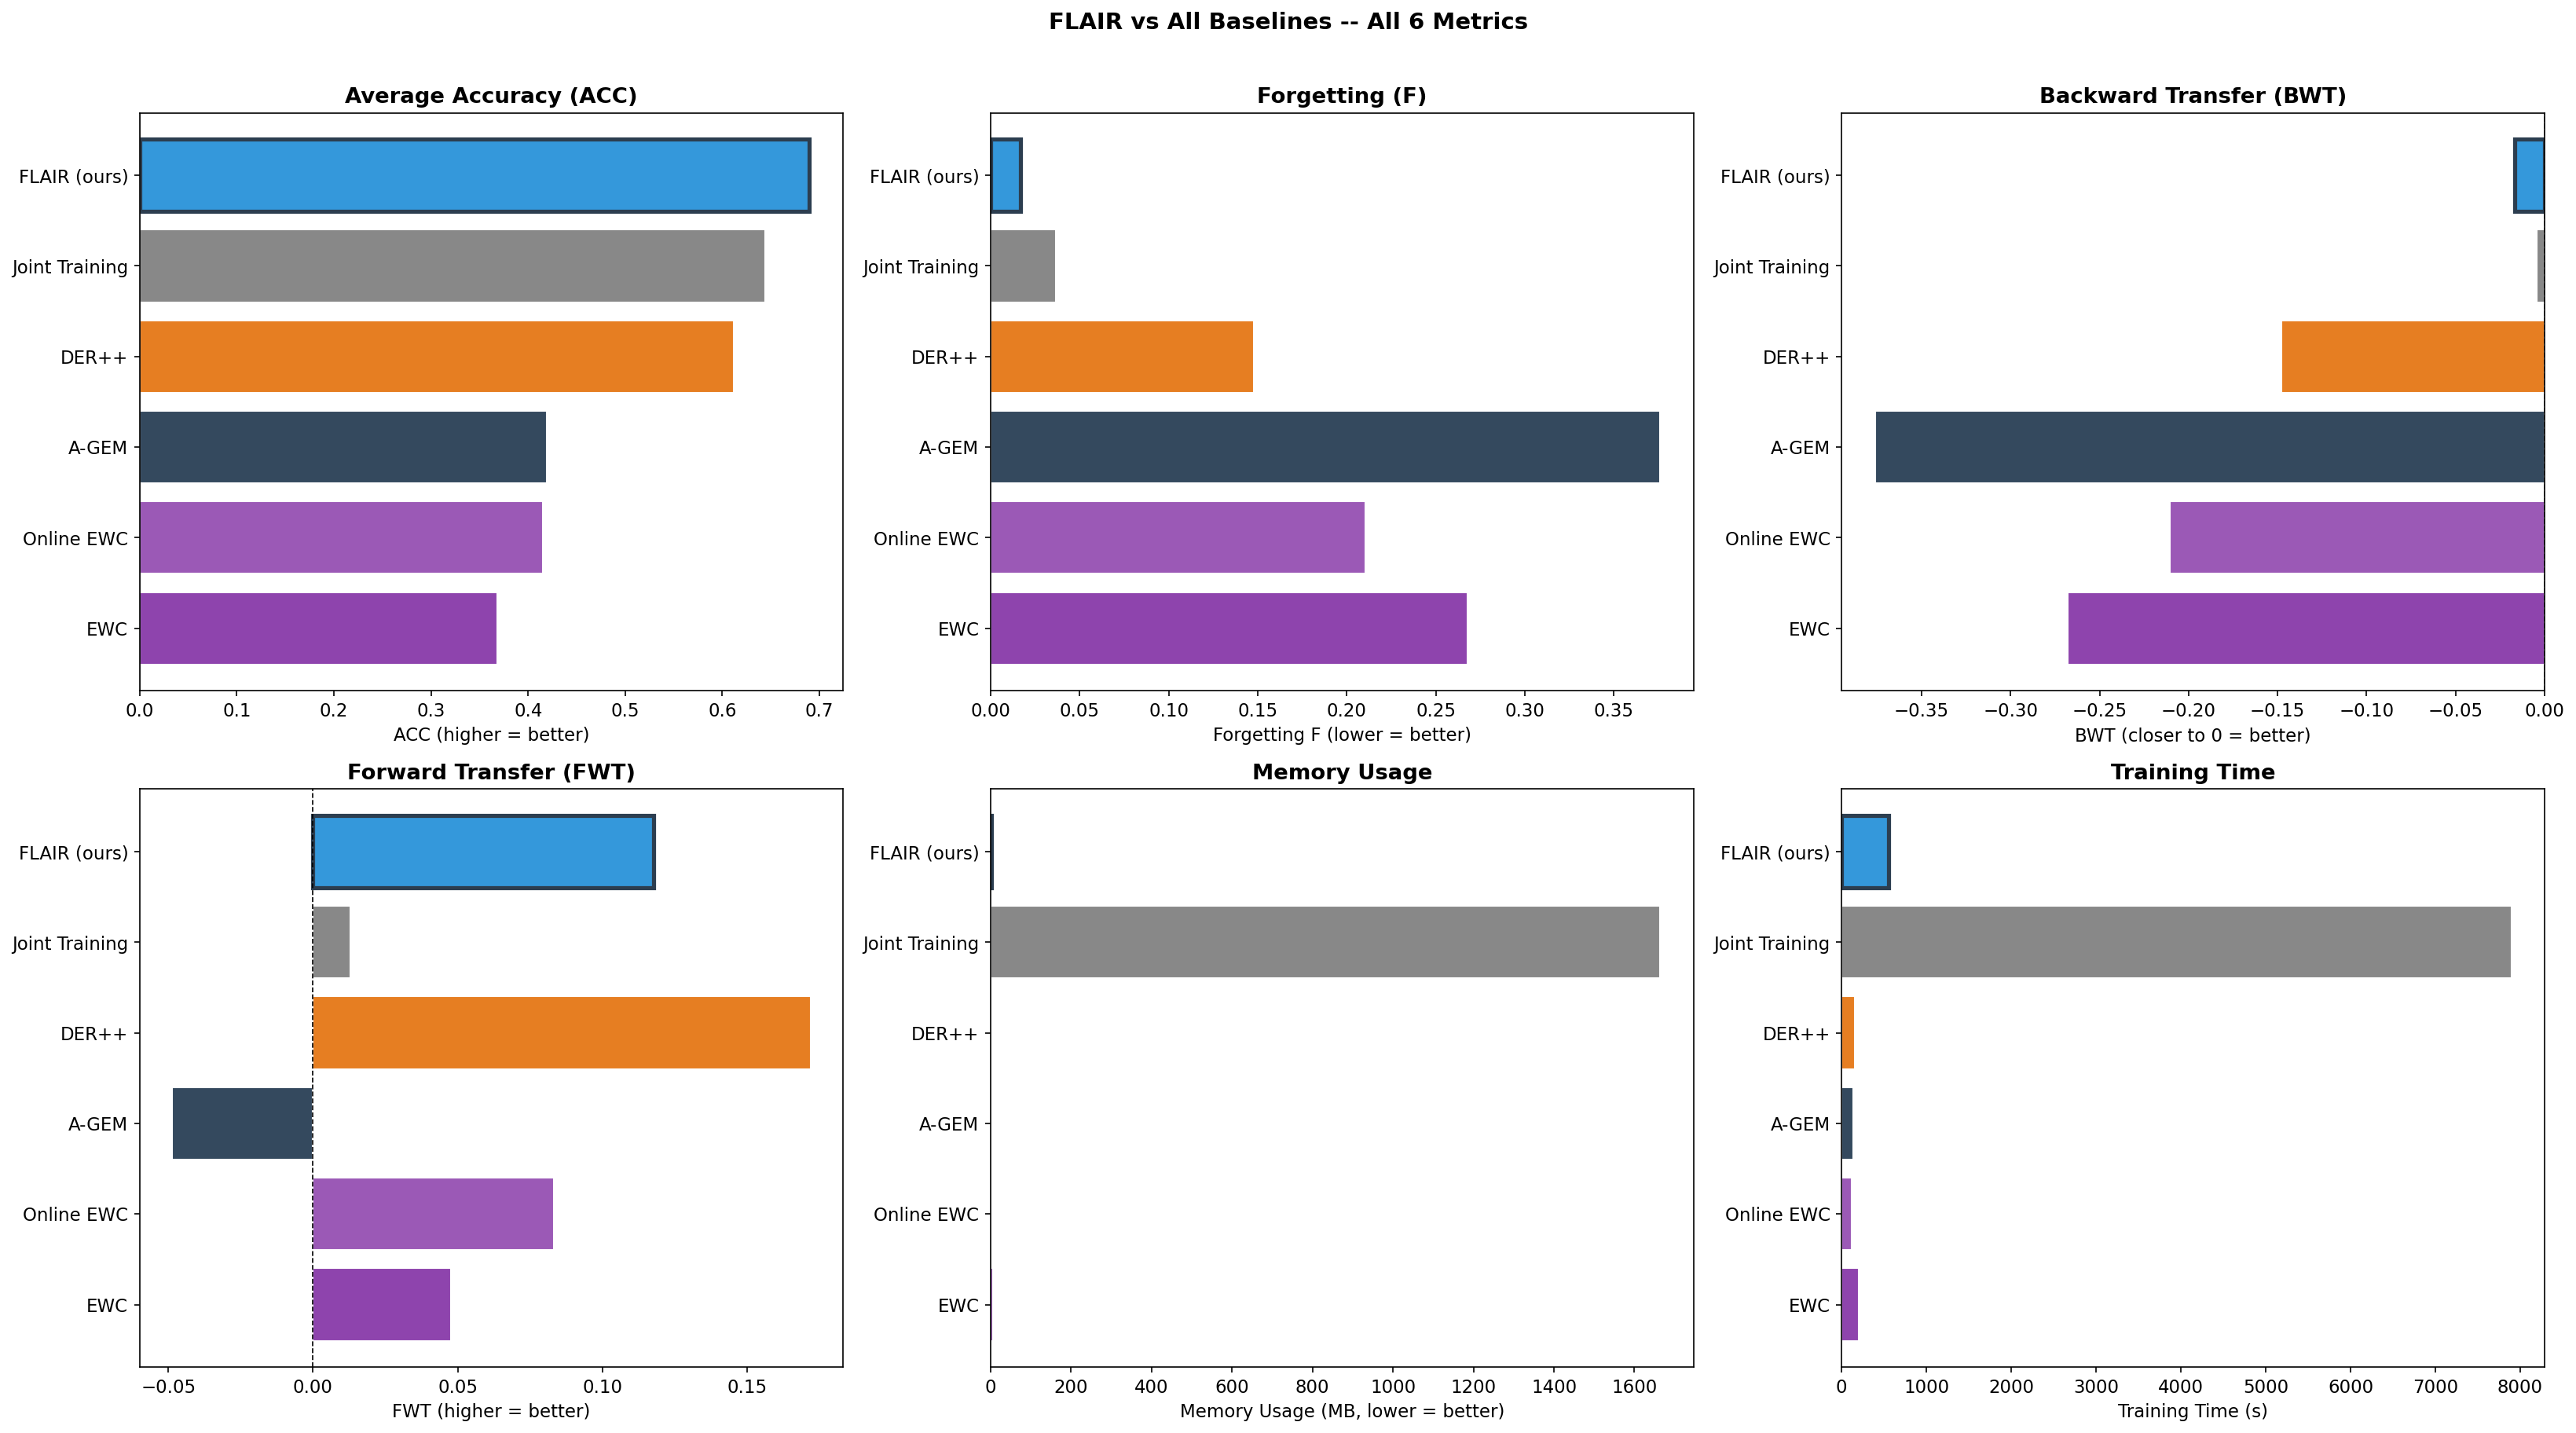
\includegraphics[width=\columnwidth]{all_metrics_comparison copy 2.png}
    \caption{Metric comparison across all methods}
    \label{fig:metrics}
\end{figure}


\subsection{Forgetting and Retention Dynamics}

Fig.~\ref{fig:forgetting} (left) tracks R\textsuperscript{2} on Task 0 as subsequent tasks are learned sequentially. FLAIR maintains 94.0\% of its initial Task 0 performance after learning 9 additional tasks (R\textsuperscript{2}: 0.768 $\rightarrow$ 0.722), compared to DER++ (81.9\%), Online EWC (46.0\%), and A-GEM (45.8\%). Joint Training shows 114.5\% retention since it retrains on all data. The right panel shows average R\textsuperscript{2} across all seen tasks over time, confirming FLAIR's stable learning trajectory.

\begin{figure}[!t]
    \centering
    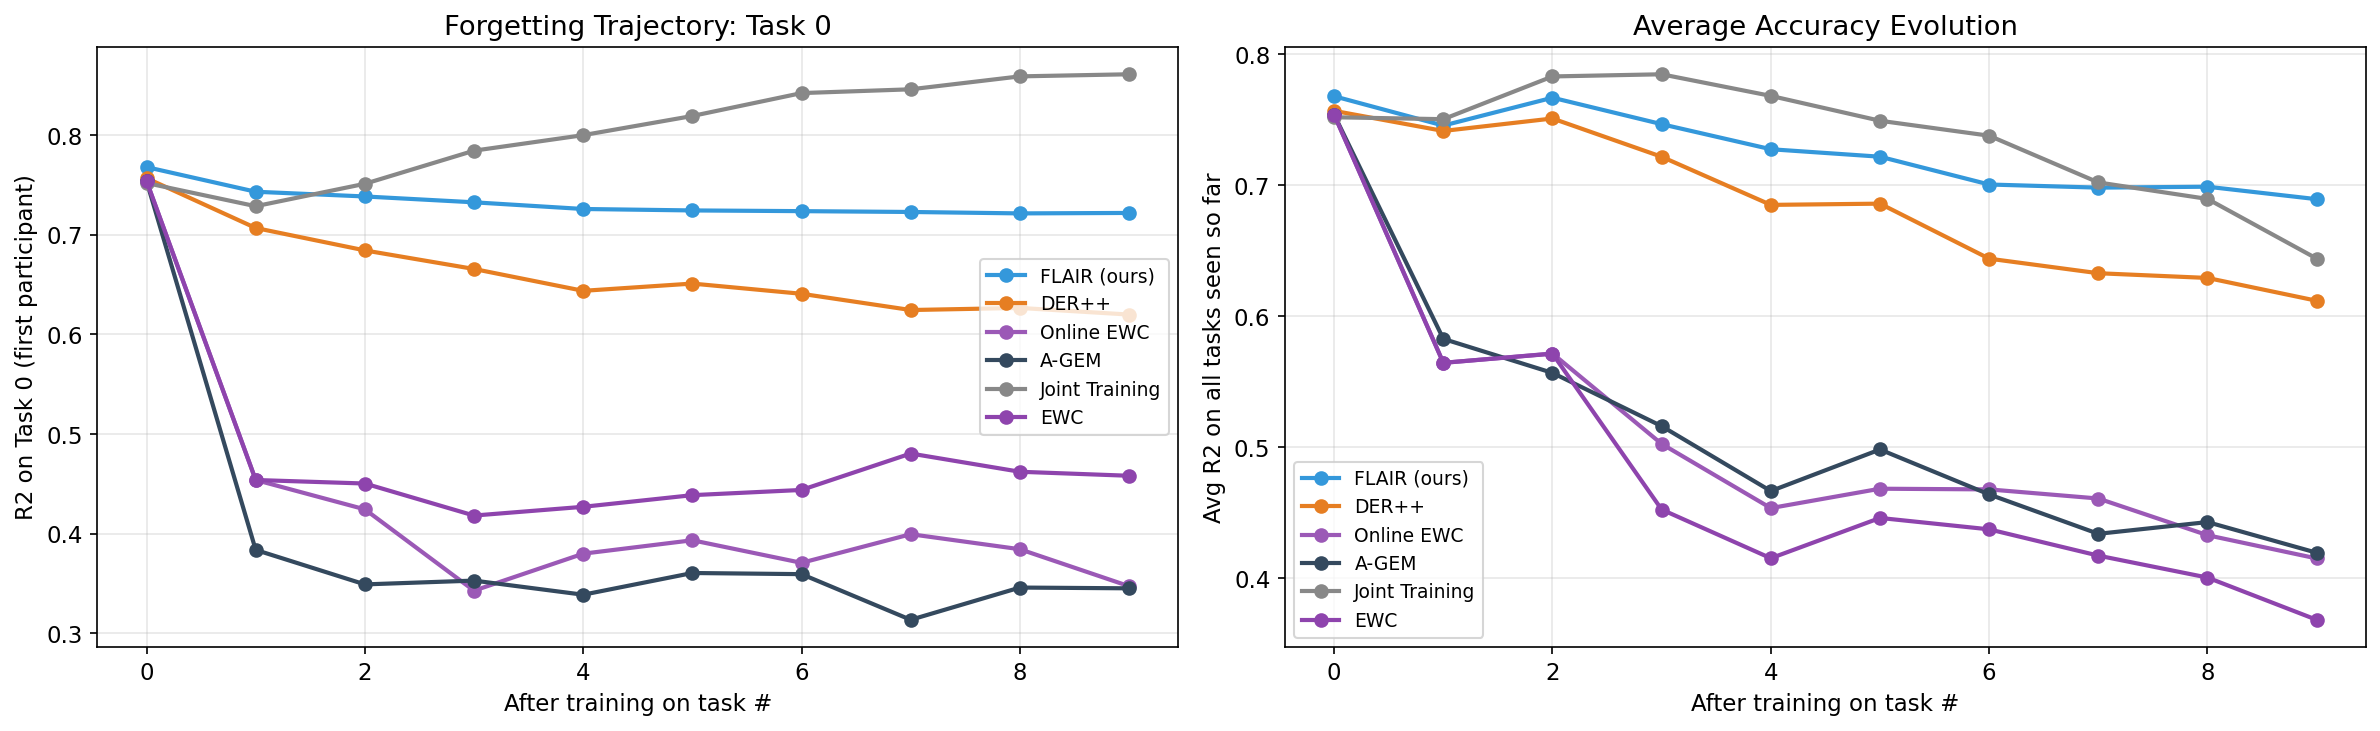
\includegraphics[width=\columnwidth]{r2_evolution copy 2.png}
    \caption{Retention dynamics across tasks}
    \label{fig:forgetting}
\end{figure}



\subsection{Per-Task Robustness}

FLAIR's R\textsuperscript{2} coefficients (performance on each task immediately after training) shows consistent quality across users: mean = 0.7047, min = 0.5770 (Task 6), max = 0.8266 (Task 2). This spread indicates heterogeneity in operator behavior, while the consistently positive and high per-task scores suggest that the model does not over-specialize to only a subset of users.

\subsection{Component Ablation}

To understand which parts of FLAIR contribute most to performance, we start from the first working FLAIR configuration and then enable individual components that address different failure modes: retroactive importance boosting, FiLM warm-start initialization, adaptive replay weighting, and blended multi-head output. Table~\ref{tab:ablation} summarizes the measured effect of each component on the sequential 10-task benchmark.

%\FloatBarrier
\begin{table}[h!]
\caption{Component ablation for FLAIR on the 10-task HRC benchmark}
\label{tab:ablation}
\centering
\footnotesize
\setlength{\tabcolsep}{4pt}
\begin{tabular}{@{}lccc@{}}
\toprule
\textbf{Configuration} & \textbf{ACC}$\uparrow$ & \textbf{F}$\downarrow$ & \textbf{BWT}$\uparrow$ \\
\midrule
Base FLAIR configuration & 0.664 & 0.039 & $-$0.039 \\
+ Retroactive importance boosting & 0.641 & 0.020 & $-$0.020 \\
+ FiLM warm-start initialization & 0.639 & 0.022 & $-$0.022 \\
+ Adaptive replay weighting & 0.636 & 0.021 & $-$0.021 \\
All FLAIR components enabled & \textbf{0.690} & \textbf{0.017} & \textbf{$-$0.017} \\
\bottomrule
\end{tabular}
\end{table}
%\FloatBarrier
The ablation shows that no single component is sufficient on its own: retroactive importance boosting, FiLM warm-start, and adaptive replay each reduce forgetting relative to the base configuration, but the full system is needed to recover the strongest final accuracy. In particular, the full FLAIR configuration improves ACC by +0.025 over the first working base model while reducing forgetting by about 2.3$\times$. This indicates that the value of FLAIR lies not in any one mechanism in isolation, but in the way FiLM conditioning, replay, and importance regularization complement one another during sequential user adaptation.

\subsection{Discussion and Practical Implications}

Joint Training is conventionally viewed as an upper bound in incremental learning, yet the observed gains of FLAIR indicate that this assumption can fail when user-specific adaptation is required: FiLM-based task conditioning provides per-user feature specialization that a single shared representation cannot capture, replay and importance regularization jointly stabilize previously learned behaviors and reduce overfitting to recent users, and warm-start initialization transfers useful structure from similar prior users to accelerate adaptation. From a deployment perspective, this combination is attractive for assistive systems because it preserves near-zero forgetting with only 1.3 MB of additional memory, avoiding the impractical cost of storing full historical datasets; although training is slower than lightweight replay-only baselines, the increased computational cost is offset by substantially better reliability across previously seen users. Overall, these results support integrated hybrid incremental designs as a more suitable strategy than single-family methods for long-horizon, multimodal HRC adaptation.

%\subsection{Limitations}

%\textbf{Single benchmark.} We evaluate only on our shared-autonomy dataset. Validation on standard CL benchmarks (e.g., Split-CIFAR, Permuted MNIST) would strengthen generalizability claims.

%\textbf{Training time overhead.} FLAIR's 3.6$\times$ slowdown versus DER++ may be a concern for time-sensitive applications, though it remains 13.8$\times$ faster than Joint Training.

%\textbf{Task identity requirement.} FLAIR requires task identity at both training and inference time (task-incremental setting). Extending to class-incremental or task-agnostic settings would require a task inference mechanism.

%===================================================================
\section{Conclusion}
%===================================================================

Assistive human-robot collaboration requires models that can continuously adapt to new users while preserving previously learned behaviors under multimodal variability and strict memory constraints. In this setting, relying on only one incremental learning strategy is often insufficient to balance plasticity and stability.

To address this challenge, FLAIR is introduced as a unified hybrid incremental learning algorithm built to maintain a stable long-term balance between plasticity and memory retention, so the system can keep learning in realistic assistive HRC without losing earlier collaboration skills.

On a sequential multimodal benchmark, FLAIR achieves better results over other methods, outperforming established ICL baselines and the Joint Training upper bound. These results indicate that combining complementary mechanisms in a single framework is an effective strategy for robust user adaptation in assistive robotics. 

Further validation on additional benchmarks would strengthen these findings and help define future research directions.

% Add acknowledgments here.
\newpage
\bibliographystyle{elsarticle-num}
\bibliography{references}

\end{document}
